\begin{answer}
\begin{figure}[H]
	\centering
	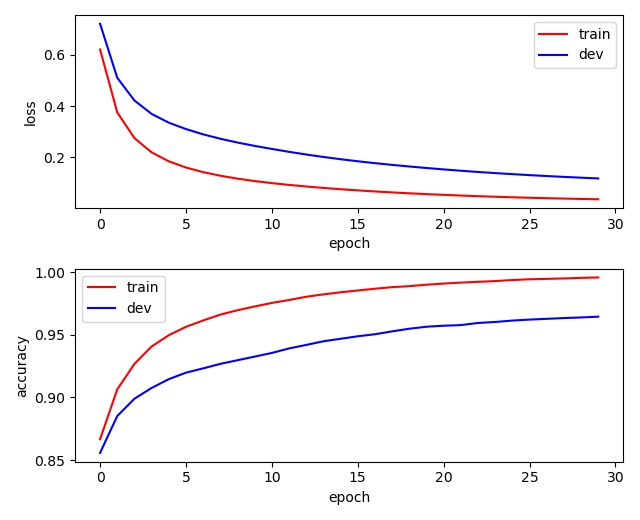
\includegraphics[width=0.6\linewidth]{regularized}
	\caption{Regularized NN model.}
\end{figure}
These model attained the same level of accuracy on the training set which was actually almost optimal. But the gap from the training to the dev accuracy is greater in the non-regularized baseline model. As a heuristic, this characteristic might indicate that compared to the regularized model, the baseline endured larger variance problem. Regularization did help in this case. And we expect better test accuracy on the second model (as we will see in the next sub-problem). \\
\end{answer}

   
  
